% Metódy inžinierskej práce

\documentclass[10pt,oneside,slovak,a4paper]{article}
\usepackage {float}
\usepackage[slovak]{babel}
%\usepackage[T1]{fontenc}
\usepackage[IL2]{fontenc} % lepšia sadzba písmena Ľ než v T1
\usepackage[utf8]{inputenc}
\usepackage{graphicx}
\usepackage{url} % príkaz \url na formátovanie URL
\usepackage{hyperref} % odkazy v texte budú aktívne (pri niektorých triedach dokumentov spôsobuje posun textu)

\usepackage[table,xcdraw]{xcolor}
\usepackage{cite}
%\usepackage{times}

\pagestyle{headings}

\title{Vývin inovatívnej platformy e-learningu pre nepočujúcich\thanks{Semestrálny projekt v predmete Metódy inžinierskej práce, ak. rok 2020/21, vedenie: Ing. Jozef Sitarčík}} % meno a priezvisko vyučujúceho na cvičeniach

\author{Petra Hlavinová\\[2pt]
	{\small Slovenská technická univerzita v Bratislave}\\
	{\small Fakulta informatiky a informačných technológií}\\
	{\small \texttt{xhlavinova@stuba.sk}}
	}

\date{\small 15. október 2020} % upravte



\begin{document}

\maketitle

\begin{abstract}
E-learning je čoraz viac atraktívnejším nástrojom pre študentov. Vďaka neustálemu rozširovaniu inteligentných zariadení a modernej technológie sa stáva učenie a získavanie informácií stále jednoduchšie a rýchlejšie. Práve pre nepočujúcich študentov môže mať e-learning množstvo výhod, no napriek tomu čelí táto skupina so špecifickými vzdelávacími potrebami v dnešnej dobe mnohým prekážkam v prístupe ku vzdelávaniu. V tejto štúdii sme sa zamerali na skúmanie týchto prekážok, spôsobu, akým sa nepočujúci učia, ako aj na to, ako by im mali byť prezentované informácie a najmä vzdelávací obsah. Naším cieľom bolo analyzovať kognitívne vlastnosti nepočujúcich a hlavne nájsť a vyvinúť inovatívnu a užívateľský prívetivú platformu e-learningu vhodnú pre potreby nepočujúcich študentov. 
\end{abstract}

\section{Úvod}

Zdá sa, že nepočujúci ľudia sú v dnešnej dobe stále do veľkej miery sociálne vylúčení. Sociálne vylúčenie nepočujúcich je podmienené viacerými faktormi, či už vzdelávacím systémom, právnymi predpismi v sociálnej oblasti a postojmi ľudí v spoločnosti. Paradoxne však práve celoživotné vzdelávanie predstavuje rozhodujúci parameter proti sociálnemu vylúčeniu nepočujúcich ľudí. Vznik e-learningu uľahčil a stále uľahčuje vzdelávanie sa ľuďom na celom svete. Vplyvu internetu a e-learningu na skupinu sluchovo postihnutých sa budeme venovať v časti~\ref{vplyv}.

Sila internetu, a teda aj e-learning, spočíva v jeho univerzálnosti. Z toho vyplýva, že musí byť prístupný ľuďom s rôznym rozsahom sluchu, zraku, pohybu a kognitívnych schopností. V minulosti sa však zvyklo myslieť, že nepočujúcim stačí na uchopenie informácií písomný prepis zvukového obsahu. Táto metóda prepísania hovorených viet na text nie je pre nepočujúcich práve výhrou, na základe faktu, že nepočujúci ľudia majú inú úroveň čitateľských schopností. To však nie je jediný rozdiel. Práve rozdiely v kognitívnych funkciach tvoria hlavný problém pri vzdelávaní tejto cieľovej skupiny. Tomuto problému sa budeme neskôr potrebnejšie venovať v časti~\ref{rozdiely}.
 
Práve preto, aby e-vzdelávanie pokrylo túto medzeru v gramotnosti, sú potrebné kreatívne spôsoby prezentácie vzdelávacích materiálov. Téme ako na vytváranie vhodnej platformy e-learningu pre našu cieľovú skupinu sa budeme venovať v časti~\ref{navrhovanie}.


\section{Vplyv internetu na skupinu sluchovo postihnutých} \label{vplyv}

Podľa World Wide Web Consortium\footnote{World Wide Web Consortium (W3C) je medzinárodné konzorcium, ktorého členovia spoločne s verejnosťou vyvíjajú webové štandardy pre World Wide Web\cite{WWWC}.} bol internet navrhnutý tak, aby fungoval pre všetkých jednotlivcov bez ohľadu na ich schopnosti, rovnako pre ľudí  s rôznym rozsahom sluchu, zraku, pohybu ci ostatných  schopností. Vplyv internetu zásadne mení prístup k vzdelávaniu pre nepočujúcich, pretože jeho použitie \emph{odstraňuje komunikačné a interakčné bariéry}, ktorým môžu jednotlivci vo fyzickom svete čeliť. To zdôrazňuje potrebu poskytnúť ľuďom so zdravotným postihnutím príležitosti bez ohľadu na ich zdravotné postihnutie sprístupnením online služieb, najmä e-learningu, spôsobom, ktorý rešpektuje a zohľadňuje ich potreby. Nejde len o rovnaké ľudské práva, ale aj o to, aby táto technológia a jej výhody mali mať úžitok aj pre nepočujúcich a sluchovo postihnutých ľudí. Inak provokuje fenomén „digitálnej priepasti“\cite{pappas2018learning}.

\section{Nepočujúci ľudia a vzdelávanie sa} \label{vzdelanie}
Napriek univerzálnosti internetu čelí komunita nepočujúcich ľudí so špecifickými vzdelávacími potrebami v dnešnej dobe mnohým prekážkam v prístupe ku e-vzdelávaniu. Paradoxne,  však práve vzdelávanie predstavuje rozhodujúci parameter proti sociálnemu vylúčeniu nepočujúcich ľudí. 

Existujú dôkazy, že najmä pre nepočujúcich je prechod zo školy do práce omnoho ťažší ak nemajú dostatočné vzdelanie. Napriek tomu, že počet nepočujúcich študentov navštevujúcich univerzity a vysoké školy začína pomaly postupne narastať, stále musia títo študenti bojovať s rôznymi prekážkami, ktoré im bránia k prístupu k vzdelaniu.
\begin{table}[H]
\begin{tabular}{lcc}
\rowcolor[HTML]{BDD7EE}
                                                                  & Početnosť                                    & Počet percent (\%) \\
\rowcolor[HTML]{DDEBF7} 
\multicolumn{1}{c}{\cellcolor[HTML]{DDEBF7}Typ vzdelania}         & \multicolumn{1}{l}{\cellcolor[HTML]{DDEBF7}} &                    \\
Špeciálna škola                                                   & 26                                           & 49.1               \\
Bežná škola                                                       & 23                                           & 43.3               \\
Osobný asistent                                                   & 1                                            & 1.9                \\
Nič z uvedeného                                                   & 3                                            & 5.7                \\
\rowcolor[HTML]{DDEBF7} 
\multicolumn{1}{c}{\cellcolor[HTML]{DDEBF7}Nadobudnuté vzdelanie} &                                              &                    \\
Základné vzdelanie                                                & 2                                            & 3.8                \\
Stredoškolské vzdelanie                                           & 8                                            & 15.1               \\
Technické vzdelanie                                               & 6                                            & 11.3               \\
Vysokoškolské vzdelanie                                           & 37                                           & 69.8              
\end{tabular}
\centering
\end{table}

\section{Rozdiely v kognitívnych funkciách medzi nepočujúcimi a počujúcimi jedincami} \label{rozdiely}
Vývin vhodnej e-learningovej platformy pre nepočujúcich by sa mal realizovať v súlade s učebným systémom, ako aj so špecifickými vzdelávacími potrebami  tejto cieľovej skupiny. Z tohto dôvodu je potrebné v prvom rade preskúmať hlavné rozdiely v kognitívnych schopnostiach medzi nepočujúcimi a počujúcimi jedincami.\linebreak
Tieto rozdiely môžeme rozdeliť do nasledovných sfér:
\begin{itemize}
\item ~\ref{rozdiely:vseob} Všeobecný kognitívny profil
\item ~\ref{rozdiely:pozornost} Pozornosť
\item ~\ref{rozdiely:pamat} Práca s pamäťou
\item ~\ref{rozdiely:citanie} Čítanie s porozumením
\end{itemize}



\subsection{Všeobecný kognitívny profil} \label{rozdiely:vseob}
Priemerné skóre IQ nepočujúcich je porovnateľné s počujúcimi jednotlivcami a má tendenciu sa časom zvyšovať. Nepočujúci jedinci však vykazujú rozdiely v porovnaní s počujúcimi rovesníkmi, pokiaľ ide o ich pamäť, zručnosti pri riešení problémov a akademické výsledky.

Vizuálne komunikačné schopnosti nepočujúcich, ako napríklad spracovanie vizuálneho jazyka, predstavujú individuálne kognitívne rozdiely. Uvádza sa, že nepočujúci a sluchovo postihnutí jedinci majú rovnakú úroveň citlivosti na vizuálny kontrast.

Okrem toho sa zdá, že nepočujúce deti majú poruchy jemného motorického sekvenovania, a to napriek skutočnosti, že ich vizuopriestorové kognitívne schopnosti sa výrazne nelíšia od ich sluchových vrstovníkov\cite{pappas2018learning}.


\subsection{Pozornosť} \label{rozdiely:pozornost}
Pozornosť je rozhodujúca vlastnosť pre každodenné činnosti nás všetkých. O to viac je dôležitá pre nepočujúcich jedincov, pretože identifikácia periférnych vizuálnych znakov je pre nich dôležitejšia z dôvodu straty sluchu. Strata sluchu nemusí nutne podmieniť akékoľvek problémy pozornosti, práve naopak, nepočujúci jedinci majú v porovnaní so svojimi počujúcimi rovesníkmi rovnaké a niekedy dokonca aj lepšie výsledky pri riešení úloh vyžadujúcich pozornosť. Avšak veľké rozdiely sa môžu vyskytnúť vo vizuálnej pozornosti,či v periférnej pozornosti\cite{pappas2018learning}.

Štúdia Baveliera, Dyeho a Hausera (2006) odhalila, že nepočujúci jedinci sú viac rozptýlení periférnymi rušičmi a menej centrálnymi rušičmi. \cite{bavelier2006deaf} 

\subsection{Práca s pamäťou} \label{rozdiely:pamat}
Medzi nepočujúcimi a počujúcimi jedincami existujú rozpoznateľné rozdiely pri práci s pamäťou. 

Tieto rozdiely vyplývajú zo skutočnosti, že zapamätávanie pomocou posunkového jazyka vyžaduje viac miesta v pamäti ako prostredníctvom hovoreného jazyka. Pre predstavu ako vyzerá abeceda v posunkovej reči nahliadnite na obrázok~\ref{slovenskaposunkovarec} v časti~\ref{rozdiely:posunkovyjazyk}. Posunkové jazyky však môžu mať aj negatívne vplyvy na krátkodobú pamäť kvôli ich vizuopriestorovej povahe
\cite{pappas2018learning}.

\subsection{Čítanie s porozumením} \label{rozdiely:citanie}
Nepočujúci majú nízku úroveň čitateľských schopností, pretože majú odlišný spôsob rozpoznávania slov v porovnaní s počujúcimi čitateľmi. Porozumenie textu nepočujúcich dospelých súvisí s ich čitateľskou motiváciou, a tak by práve náročné materiály na čítanie mohli postupne zlepšovať ich čitateľské schopnosti\cite{pappas2018learning}.

Domínguez a Alegria (2009) skúmali mechanizmy čítania, ktoré používajú nepočujúci dospelí. Výsledky ukázali, že väčšina účastníkov používa na pochopenie textu stratégiu kľúčových slov\cite{dominguez2010reading}. 

\subsection{Posunkový jazyk}
\label{rozdiely:posunkovyjazyk}
Nepočujúci majú k dispozícii špeciálny dorozumievací jazyk - posunkový jazyk, ktorý vo veľmi veľkej miere využíva komunita nepočujúcich ľudí. Tento jazyk využíva namiesto zvukov manuálne prostriedky komunikácie, reč tela, pohyby hlavy a hornej časti trupu.
\begin{figure}[H]
   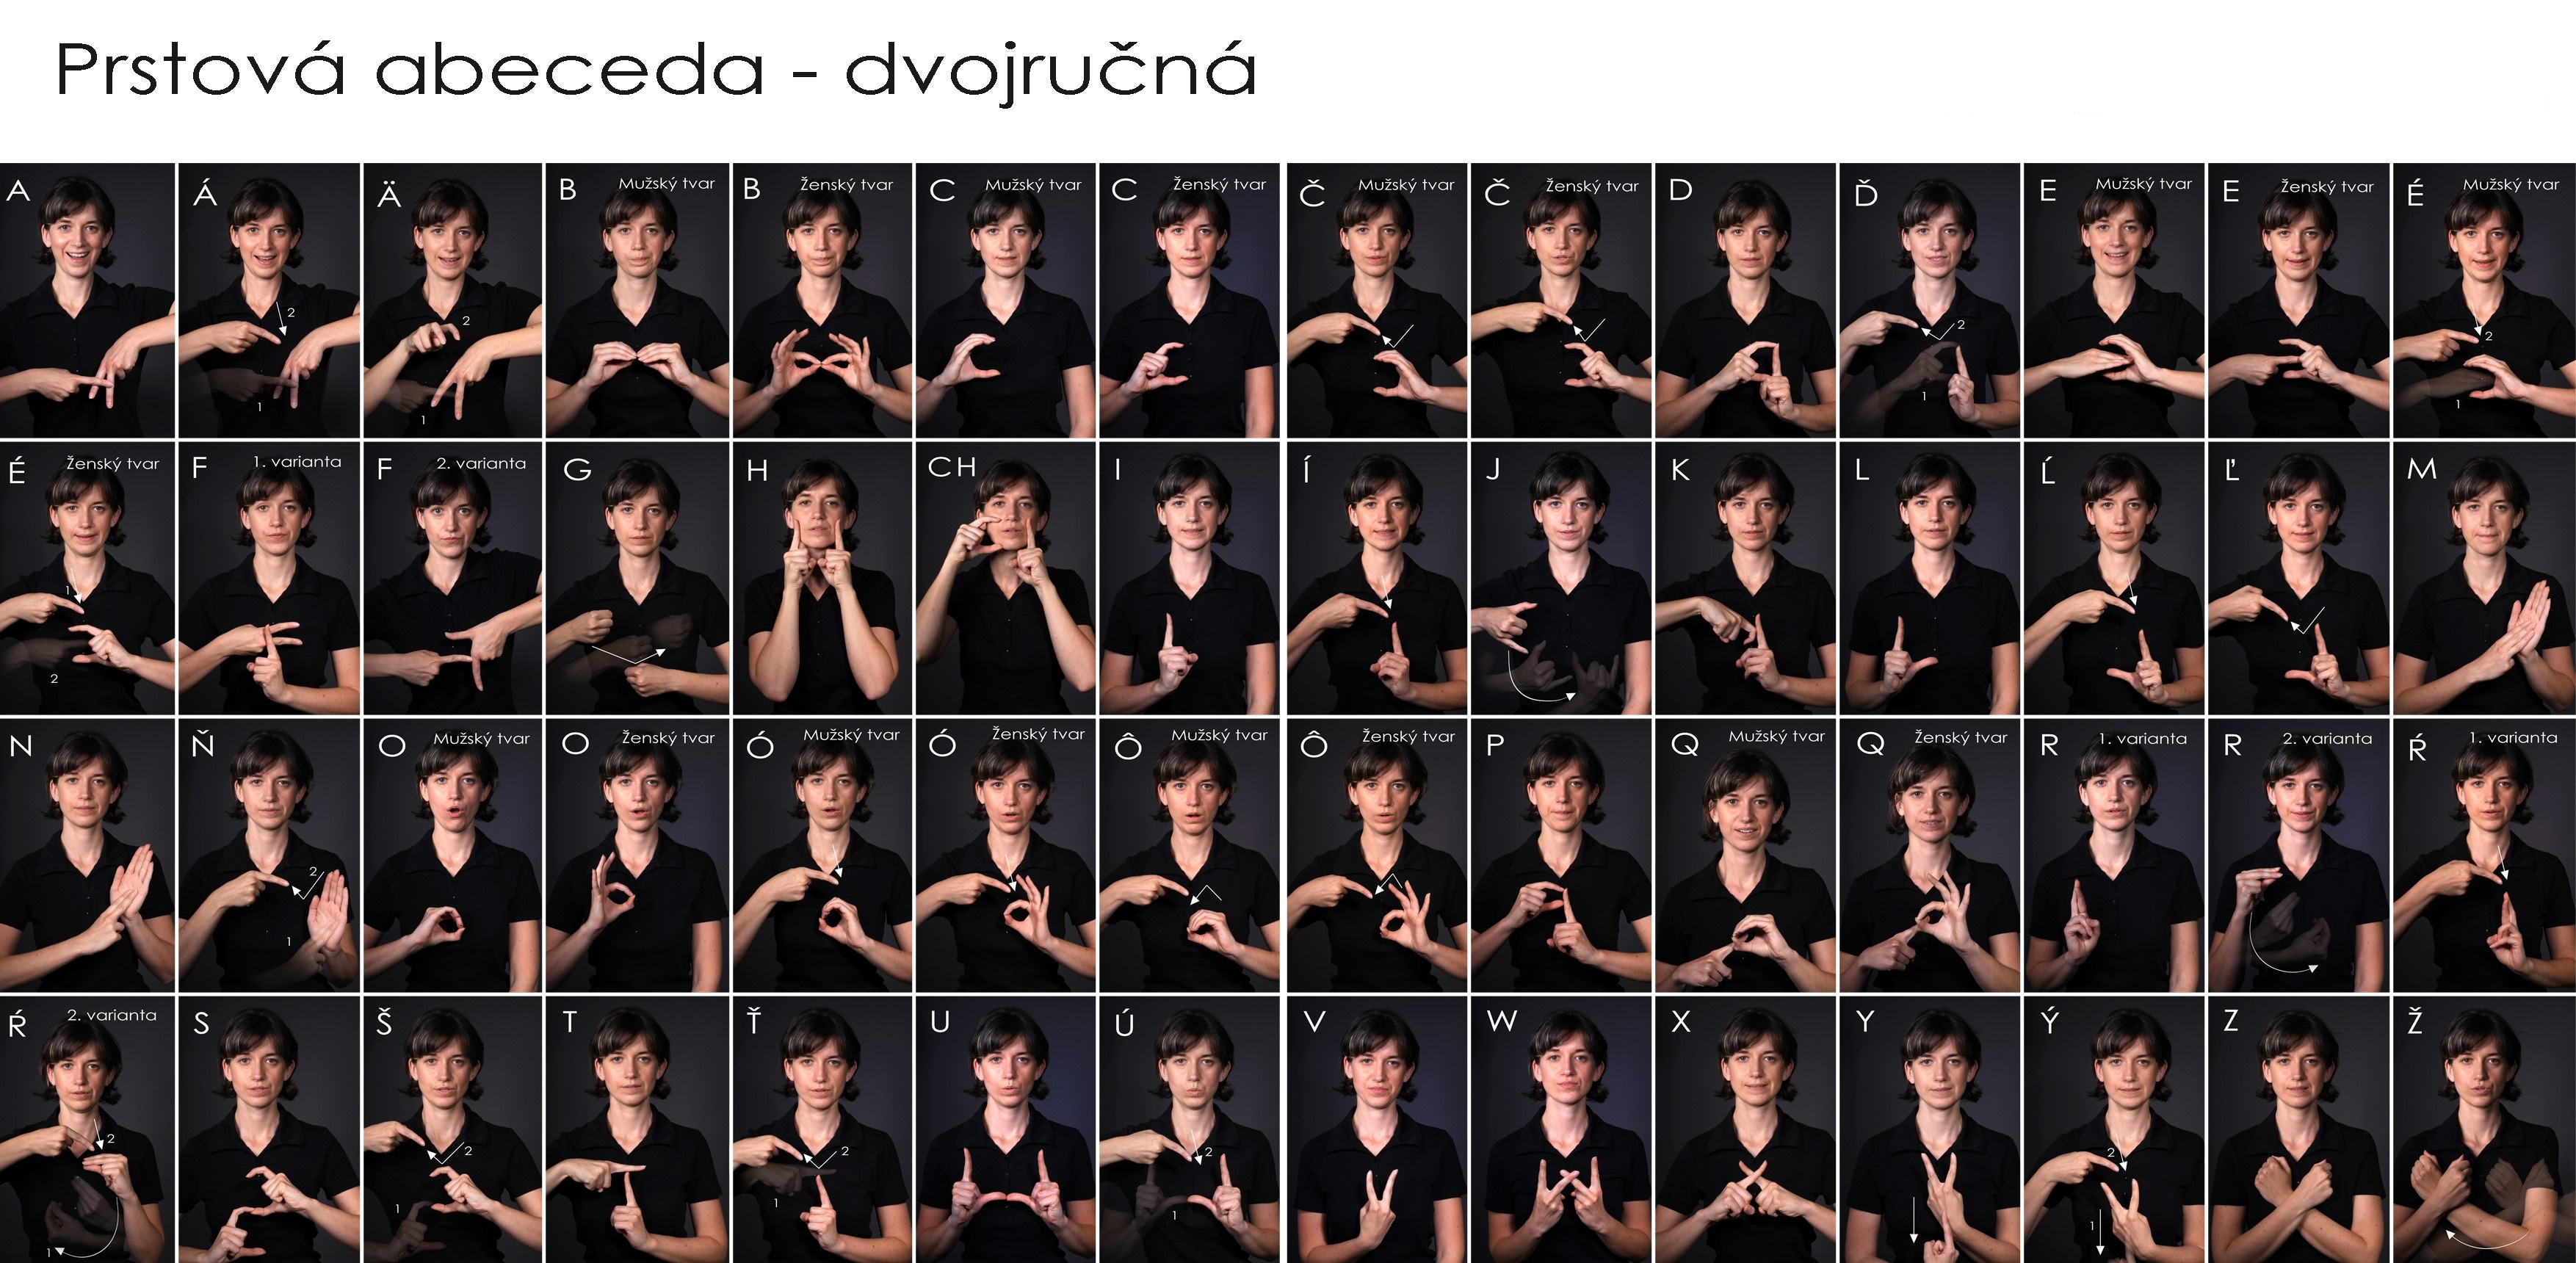
\includegraphics[scale=0.15]{dvojrucnaabeceda.jpg}
\centering
\caption{Slovenská prstová abeceda - dvojručná. Prevzaté z\cite{mytyafakty}.}

\label{slovenskaposunkovarec}
\end{figure}

\section{Navrhovanie e-learningových systémov} \label{navrhovanie}
Návrh e-learningového systému pre nepočujúcich obsahuje špecifické problémy. Takýto systém musí obsahovať prostriedky vizuálnej komunikácie a pri vzdelávaní neobvyklé formy interakcie, ako sú napríklad gestá.
\subsection{Problémy pri vytváraní e-learningových rozhraní} \label{navrhovanie:problemy}
Špeciálne vzdelávacie potreby osôb so zdravotným postihnutím, ako je hluchota a čiastočná strata sluchu, sa žiaľ dodnes pri vývoji systémov elektronického vzdelávania zohľadňujú zriedka. Je pravda, že návrh rozhraní, ktoré sú pre nich vhodné a užívateľsky prívetivé, nie je vždy ľahký proces.

Jazykové a gramotné schopnosti sa môžu líšiť v závislosti od typu a úrovne hluchoty a veku človeka, ktorý stratil sluch, a môžu byť ovplyvnené zároveň aj ich schopnosti čítania a písania. To vyvoláva ďaľšie problémy pri vytváraní e-learningových rozhraní. Projektanti takýchto systémov musia zohľadňovať špeciálne potreby cieľovej skupiny, ktoré sa vyskytujú na komunikačnej aj kognitívnej úrovni.\cite{pappas2018learning}

\subsection{Ako na to?}\label{navrhovanie:ako}
Navrhovanie e-learningových systémov pre nepočujúcich a sluchovo postihnutých jedincov vyžaduje prezentovať všetok zvuk vizuálnym spôsobom a to buď pomocou textu, titulkov, obrázkov alebo videí v posunkovej reči (Znázornené na obrázku~\ref{diagram}). Rovnako je dôležite vytvoriť vhodné grafické rozhranie, ktoré efektívne a zrozumiteľne prezentuje výučbu.
\begin{figure}[H]
   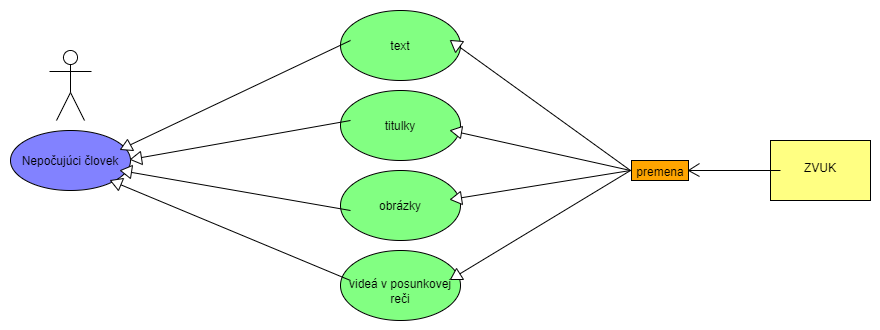
\includegraphics[scale=0.4]{diagram.png}
\centering
\caption{Diagram znázorňujúci premenu zvuku na prostriedky vhodné pre nepočujúcich}

\label{diagram}
\end{figure}

Používanie textu by sa malo obmedziť na minimum, pretože nepočujúci ľudia majú do istej miery ťažkosti s čítaním s porozumením. Štúdie napríklad ukazujú, že nepočujúci, ktorí používajú posunkovú reč, spracúvajú obrázky ľahšie a efektívnejšie v porovnaní so slovami. 

Dizajnéri a vývojári e-learningových systémov pre nepočujúcich študentov musia zohľadniť všetky vyššie uvedené parametre. \par Štúdie ukazujú, že nepočujúci, ľahšie spracovávajú obrázky v porovnaní so slovami . Medzi  najdôležitejšie metódy e-vzdelávania patria použitie príkladov, praktických otázok, či spätná väzba.. \cite{pappas2018learning}

\section{Výsledky štúdii a dotazníku} \label{dolezitejsia}
\ldots
\section{Záver} \label{zaver} % prípadne iný variant názvu
Práve v aktuálnej dobe si začíname uvedomovať 
\emph{Nie, nie je to len prepis povedanej vety na text}. Za vývinom takýchto nových platforiem stoji množstvo štúdii a riešenia mnohých komplexných problémov. Myslím si však, že za tú pomoc, ktorú to prinesie nepočujúcim študentom to naozaj stojí!.
\section{Reakcie}
\ldots
%\acknowledgement{Ak niekomu chcete poďakovať\ldots}

% týmto sa generuje zoznam literatúry z obsahu súboru literatura.bib podľa toho, na čo sa v článku odkazujete
\bibliography{literatura}
\bibliographystyle{plain} % prípadne alpha, abbrv alebo hociktorý iný
\end{document}
